\title{CW1: An Unknown Signal}
\date{\today}

\documentclass[12pt]{article}

\usepackage{graphicx}
%\usepackage{minted}

\renewcommand{\today}{\ifcase \month \or January\or February\or March\or %
April\or May \or June\or July\or August\or September\or October\or November\or %
December\fi, \number \year} 

\author{Michael Wray \& Davide Moltisanti}

\begin{document}
\maketitle

\section{Introduction}
\label{sec:intro}
The year is 1983, the strategy of D\'etente (de-escalation via verbal agreement) has failed.
Both the United States of America and the Soviet Union have been stockpiling nuclear weapons and recent political events have brought the world on the cusp of total annihilation.
As an operator for a nuclear early warning device you receive an unknown signal... 

\section{Task}
\label{sec:task}
In this coursework you will be given example points which follow an unknown signal.
You will be required to reconstruct the signal and give the resulting error.
Your solutions will be auto-marked with a variety of different inputs in order to test both the correctness and robustness of your system. 

\section{Implementation}
\label{sec:implementation}
Your final solution will use the linear least squares regression code that you have created in the worksheets which will need to be extended in order to cope with non-linear curves.
Your solution should:
\begin{itemize}
    \item Read in a file containing a number of different line segments (each made up of 20 points)
    \item Determine the function type of line segment, \textit{e.g.} linear/polynomial/unknown function (there is one unknown function), using least squares regression 
    \item Produce the total reconstruction error 
    \item Produce a figure showing the reconstructed line from the points if an optional argument is given. 
\end{itemize}

\paragraph{Note:} All Code written for the least squares regression sections must be written by yourself.
Any calls to Scipy's regression solver or any other similar library are forbidden and will be treated as \textbf{not implemented}.

\section{Marks}
\label{sec:marks}
Each solution will go through 50 tests in order to test its correctness and robustness.
These test files will be similar in nature to the train files that you have been provided.
Each test will be worth 2 points broken down as the following: 
\begin{itemize}
    \item 0: Solution gave incorrect output format and/or didn’t finish execution. 
    \item 1: Solution gave correct output format but a large error difference. 
    \item 2: Solution gave correct output format and a small error difference. 
\end{itemize}
\paragraph{Note:} The ‘error difference’ will be the difference in error between your solution and a model solution we have coded.
This will be different for every test and more information will be provided when the marks are released. 

\subsection{Up to $40\%$}
Solutions which have implemented the linear least squares regression.

\subsection{Up to $60\%$}
Solutions with an extended least squares regression to handle polynomial inputs with few errors.

\subsection{Up to $80\%$}
Solutions with an extended least squares regression fine-tuned to the output signal which fail on edge cases.

\subsection{Up to $100\%$}
A perfect solution that reconstructs every signal with minimum error.


\section{Train/Test Files}
\label{sec:train_files}
The input files are Comma Separated Value (CSVs) which consists of two columns for the x and y dimensions respectively.
Each input file will be split into different line segments each made up of 20 different points, so the first 20 points correspond to the first line segment, 21-40 the second line segment \textit{etc}.
Two consecutive line segments may/may not follow the same trend.
A line segment will follow a linear, polynomial or another unknown function.
An example train file is given below (basic\_2.csv): 

\begin{verbatim}
    \small
    -2.9251047704944395,4.8735802196928955
    -0.8554275589011144,8.298220787115126
    0.19855925795710938,10.042225113162727
    0.43421216060191,10.432153786922873
    0.624770694735732,10.747465992520771
    1.3614382007711343,11.96641038237006
    1.5943359027154818,12.351780097835984
    4.194060135884697,16.653475561819924
    4.6779257660237565,17.45411532191076
    5.023596843152395,18.026088181779052
    7.288865840413205,21.774369344024162
    7.485381750603618,22.099539063443302
    7.932320124145074,22.839076261125182
    9.697898711534522,25.760532815546593
    9.79296969415338,25.91784427553536
    10.338531977763036,26.820571869016863
    10.47247053028027,27.042196476913674
    11.373020960538451,28.532313640689885
    12.448760928878032,30.31231233562508
    12.518847008701732,30.428281932638267
    12.653923639452994,30.27170891389091
    12.717363846157376,30.149430959474596
    12.922893495415568,29.753282422312626
    13.82087982807715,28.02245685354787
    16.940698414027672,22.009156225167718
    17.888369346145012,20.182565974932835
    19.383541905873596,17.300692607859034
    19.669839705150725,16.748867336976346
    20.098166635136398,15.923287731535833
    20.564236539021604,15.024960354898298
    20.621376796845194,14.914825249663732
    21.505205350325678,13.211288120947877
    27.70770290983017,1.2562716850382856
    28.51062072023851,-0.2913138686887322
    28.664485990065593,-0.5878817934724623
    29.937739282405232,-3.042016420848668
    30.093442528905104,-3.3421269574788823
    30.886445731764947,-4.870602580881737
    31.512235111191547,-6.076781582919168
    31.755689686592167,-6.546028595495876
\end{verbatim}

This corresponds to 40 points of x and y co-ordinates which make up the two different line segments of the file. 
Test files could consist of any number of line segments (\textit{i.e.} longer than adv\_3.csv) as well as have large amounts of noise. 

\section{Input/Output}
\label{sec:IO}

The auto-marker will expect a program called \textbf{lsr.py} (\textbf{not a jupyter notebook}) which will be run as follows:
\begin{verbatim}
    $ python lsr.py test_2.csv
\end{verbatim}

After execution your program should print out the total reconstruction error, created by summing the error for every line segment, followed by a newline character:

\begin{verbatim}
    $ python lsr.py basic_2.csv
    6.467081701001855e-27
    $
\end{verbatim}

Additionally, to further understand and validate your solution we wish for your program to be able to visualise the result given an optional parameter, \texttt{--plot}.
This is only to visually check that your solution is working and will not be part of the automarker (styling of the plot itself doesn't matter).
For example, running:

\begin{verbatim}
    $ python lsr.py basic_2.csv --plot
    6.467081701001855e-27
\end{verbatim}

Will also show the following visualisation:

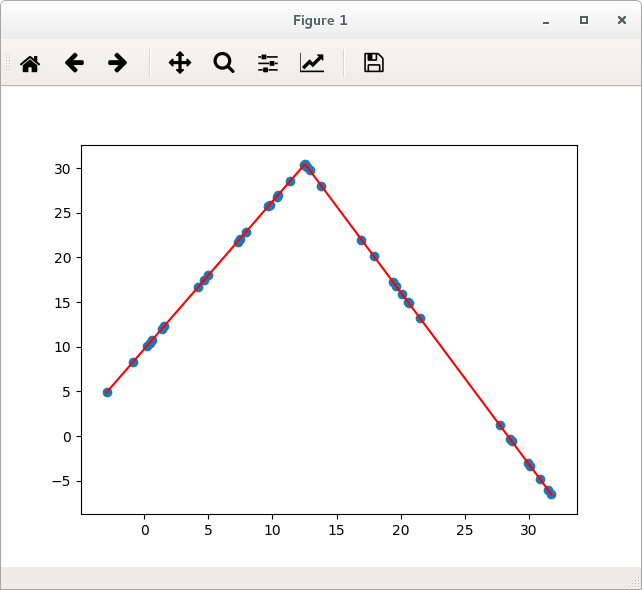
\includegraphics[width=0.65\textwidth]{CW1_visualisation}

Note the presence of both the original points (blue dots) and fitted line segments (red lines).

\section{Hints/Notes}
\label{sec:hints/notes}
\begin{itemize}
    \item We have provided you a utilities file which contains two functions: \textit{load\_points\_from\_file} and \textit{view\_data\_points}.
        The first will load the data points from a file and return them as two numpy arrays.
        The second will visualise the data points with a different colour per segment.
    \item The error you need to calculate is the sum squared error. 
    \item Regardless of the number of segments your program needs to only output the total reconstruction error. 
    \item The test files will include points approximating line segments generated from the three functions mentioned above, \textit{i.e.} linear, polynomial or the unknown function. 
    \item The order of the polynomial function \textbf{will not} change between the train files and the test files.
    \item Having a very low error might not be the correct answer to a noisy solution, refer to overfitting in the lecture slides. 
\end{itemize}
\end{document}
